%%%%%%%%%%%%%%%%%%%%%%%%%%%%%%%%%%%%%%%%%%
\section{Results and conclusion}
\label{chaper_results}

A two-dimensional (2D) unbinned maximum-likelihood fit to the $m_{\mu^{+}\mu^{-}\gamma}$ and $m_{\mu^{+}\mu^{-}}$ distributions was used to compare the data with background and signal predictions. Search has been performed for a SM Higgs and $\mathrm{Z}$ boson decaying into a $\Upsilon(1S,2S,3S)\gamma$, with $\Upsilon(1S,2S,3S)$ subsequently decaying into $\mu^{+}\mu^{-}$ using data obtained from $35.9~fb^{-1}$ of $pp$ colisions at $\sqrt{s}=13~\mathrm{TeV}$. 

Since no excess has been observed above the background, the \CLs formalism is applied, in order to establish an upper limit in the branching fractions for each channel.

\subsection{The $CL_{s}$ formalism for upper limits setting at CMS}
\label{sec:cls}

The \CLs formalism~\cite{cls_Read_2002} consist in a modified frequentist approach to obtain an upper limit for a certain parameter of a model, with respect to the data, when there is no significant excess that could justify an observation. It is based on the profile-likelihood-ratio test statistic~\cite{profiled_lh} and asymptotic approximations~\cite{asymptotic_cls}. It is a standard upper limit setting procedure for the LHC experiments~\cite{CMS-NOTE-2011-005}.

When searching for non-observed phenomena, it is often usual to derive the results as a function of the signal strength modifier $\mu$, which is a free parameter of the full model (signal + background). It can be defined such as, the expectation value for the number of events in a bin~\footnote{A set of common analysis criteria.} is:


\begin{equation}
\label{eqn:signal_strength}
E[n] = \mu s + b,
\end{equation}
where, $s$ and $b$ are the expected number of signal and background events, respectively.

The Neyman–Pearson lemma~\cite{profiled_lh} states the likelihood ratio is the optimal test between a null hypothesis and an alternative one (i.e. background-only and signal-plus-background models). On top on this, one could build a likelihood ratio test as:


\begin{equation}
  \label{profile_likelihood_ratio_lep}
  q(\mu)=-2ln \left(\frac{ \mathcal{L}(\text{data} \vert \mu s + b) }{\mathcal{L}(\text{data} \vert b)} \right),
\end{equation}
  where the denominator and numerator defines the likelihoods for the background-only and signal-plus-background models, respectively. The was the hypothesis test used by LEP and Tevatron experiments (the former one, with some modifications to include the nuisances effects).

With these two models, i.e. their \textit{pdfs}, one can throw toy MC events in order to construct a distribution of $q(\mu)$, namely $f(q(\mu) \vert \mu)$. The $p$-value of $f(q(\mu) \vert \mu)$, as below, can be used to chose between each model.

\begin{equation}
  \label{p_value_lep}
  p_{\mu}=\int^{\infty}_{q(\mu)_{\text{data}}} f(q(\mu) \vert \mu) \text{ } dq(\mu),
\end{equation}
  where $q(\mu)_{\text{data}}$ is the observed value of $q(\mu)$ on data, for a given $\mu$. 
  
If $p_{\mu}$ is less than $\alpha$ (usually 0.05 or 0.1) the background-only model can be excluded in favor of the signal-plus-background model. For the purpose of a confidence interval estimation, the argument can be reversed and one could look for all the values of $\mu$ that would not be excluded with Confidence Level (CL) $1-\alpha$.

The problem with this definition is that, when the expected signal strength is very small, e.g. a invariant mass distribution in the TeV scale, the null hypothesis and the alternative one are almost indistinguishable. In this situation, a downward fluctuation of the background might lead us to exclude the alternative hypothesis (signal) in a region of low experimental sensitivity region. Putting in number, if we expect 50 background events and 2 signal events, but we observe 40 events, the signal would be easily excluded.

In order to take this effect into account, a modified frequentist approach for upper limits setting, the $CL_s$ was proposed during the Higgs search era at LEP. Lets start by considering a profile likelihood ratio~\cite{kendall} as below:


\begin{equation}
  \label{profile_likelihood_ratio_def}
  \lambda(\mu)=\frac{ \mathcal{L}(\text{data} \vert \mu, \doublehat{\theta}) }{\mathcal{L}(\text{data} \vert \hat{\mu}, \hat{\theta})},
\end{equation}
  where, $\mathcal{L}(\text{data} \vert \mu, \doublehat{\theta})$ is the profile likelihood function. 

Defining $\mu$ and the investigated signal strength, $\doublehat{\theta}$ is the nuisances that maximizes the likelihood for a given $\mu$ (fixed) while $\hat{\mu}$ and $\hat{\theta}$ are the signal strength and nuisances that, overall, maximizes the likelihood. The advantage of the CMS and ATLAS have a common set of statistical guidelines~\cite{cms_atlas_statistical_guidelines} to ensure the compatibility of the published results. Following these recommendations, the statistics test based on~\ref{profile_likelihood_ratio_def} is:

\begin{equation}
  \label{statistics_test_lhc}
  \tilde{q_{\mu}}=-2 ln[\lambda(\mu)], \text{ with } 0 \leqslant \hat{\mu} \leqslant \mu.
\end{equation}

The left side restriction ($0 \leqslant \hat{\mu}$) ensure us the proper physical interpretation of $\mu$ as a positive defined signal strength, i.e., the observation a process would, for a given bin, increase the number of events. The right side restriction $\hat{\mu} \leqslant \mu$ secure the interpretation of $\tilde{q_{\mu}}$'s $p-$value as a one-sided confidence interval. This is required for a upper limit definition.

The advantage of using the profile likelihood ratio is that, even though it takes into account the effect of nuisances in the likelihood, it is possible to prove that, with the use of Wilk's Theorem~\cite{wilks1938}, that a statistic test defined as $\tilde{q_{\mu}}$, asymptotically follows a chi-square distribution with one degree of freedom (the signal strength)~\cite{asymptotic_cls}. Thus, $\tilde{q_{\mu}}$ is said to be approximately independent of any nuisance and allow a fast computation of its $p$-value without the need of toy MC strategies (which can computationally demanding, depending on the complexity of the models), event though this is not the standard CMS/ATLAS recommendation.

Based on $\tilde{q_{\mu}}$, defined at~\ref{statistics_test_lhc}, one should compute the $\tilde{q_{\mu}}^{\text{obs}}$,also the $\hat{\theta}_{\mu}^{\text{obs}}$ and $\hat{\theta}_{\mu = 0}^{\text{obs}}$, which corresponds to the observed value of $\tilde{q_{\mu}}$ on data, the maximum likelihood estimator for the nuisances assuming some signal strength $\mu$ and assuming a background-only model, respectively. Then, the distributions of $f(\tilde{q_{\mu}} \vert \mu, \hat{\theta}_{\mu}^{\text{obs}})$ and $f(\tilde{q_{\mu}} \vert \mu=0, \hat{\theta}_{\mu = 0}^{\text{obs}})$ are generated tossing pseudo-random toy MC. Figure~\ref{toy_mc_profile_likelihood_test} presents an example of these two distributions.

\begin{figure}[htbp]
  \centering
  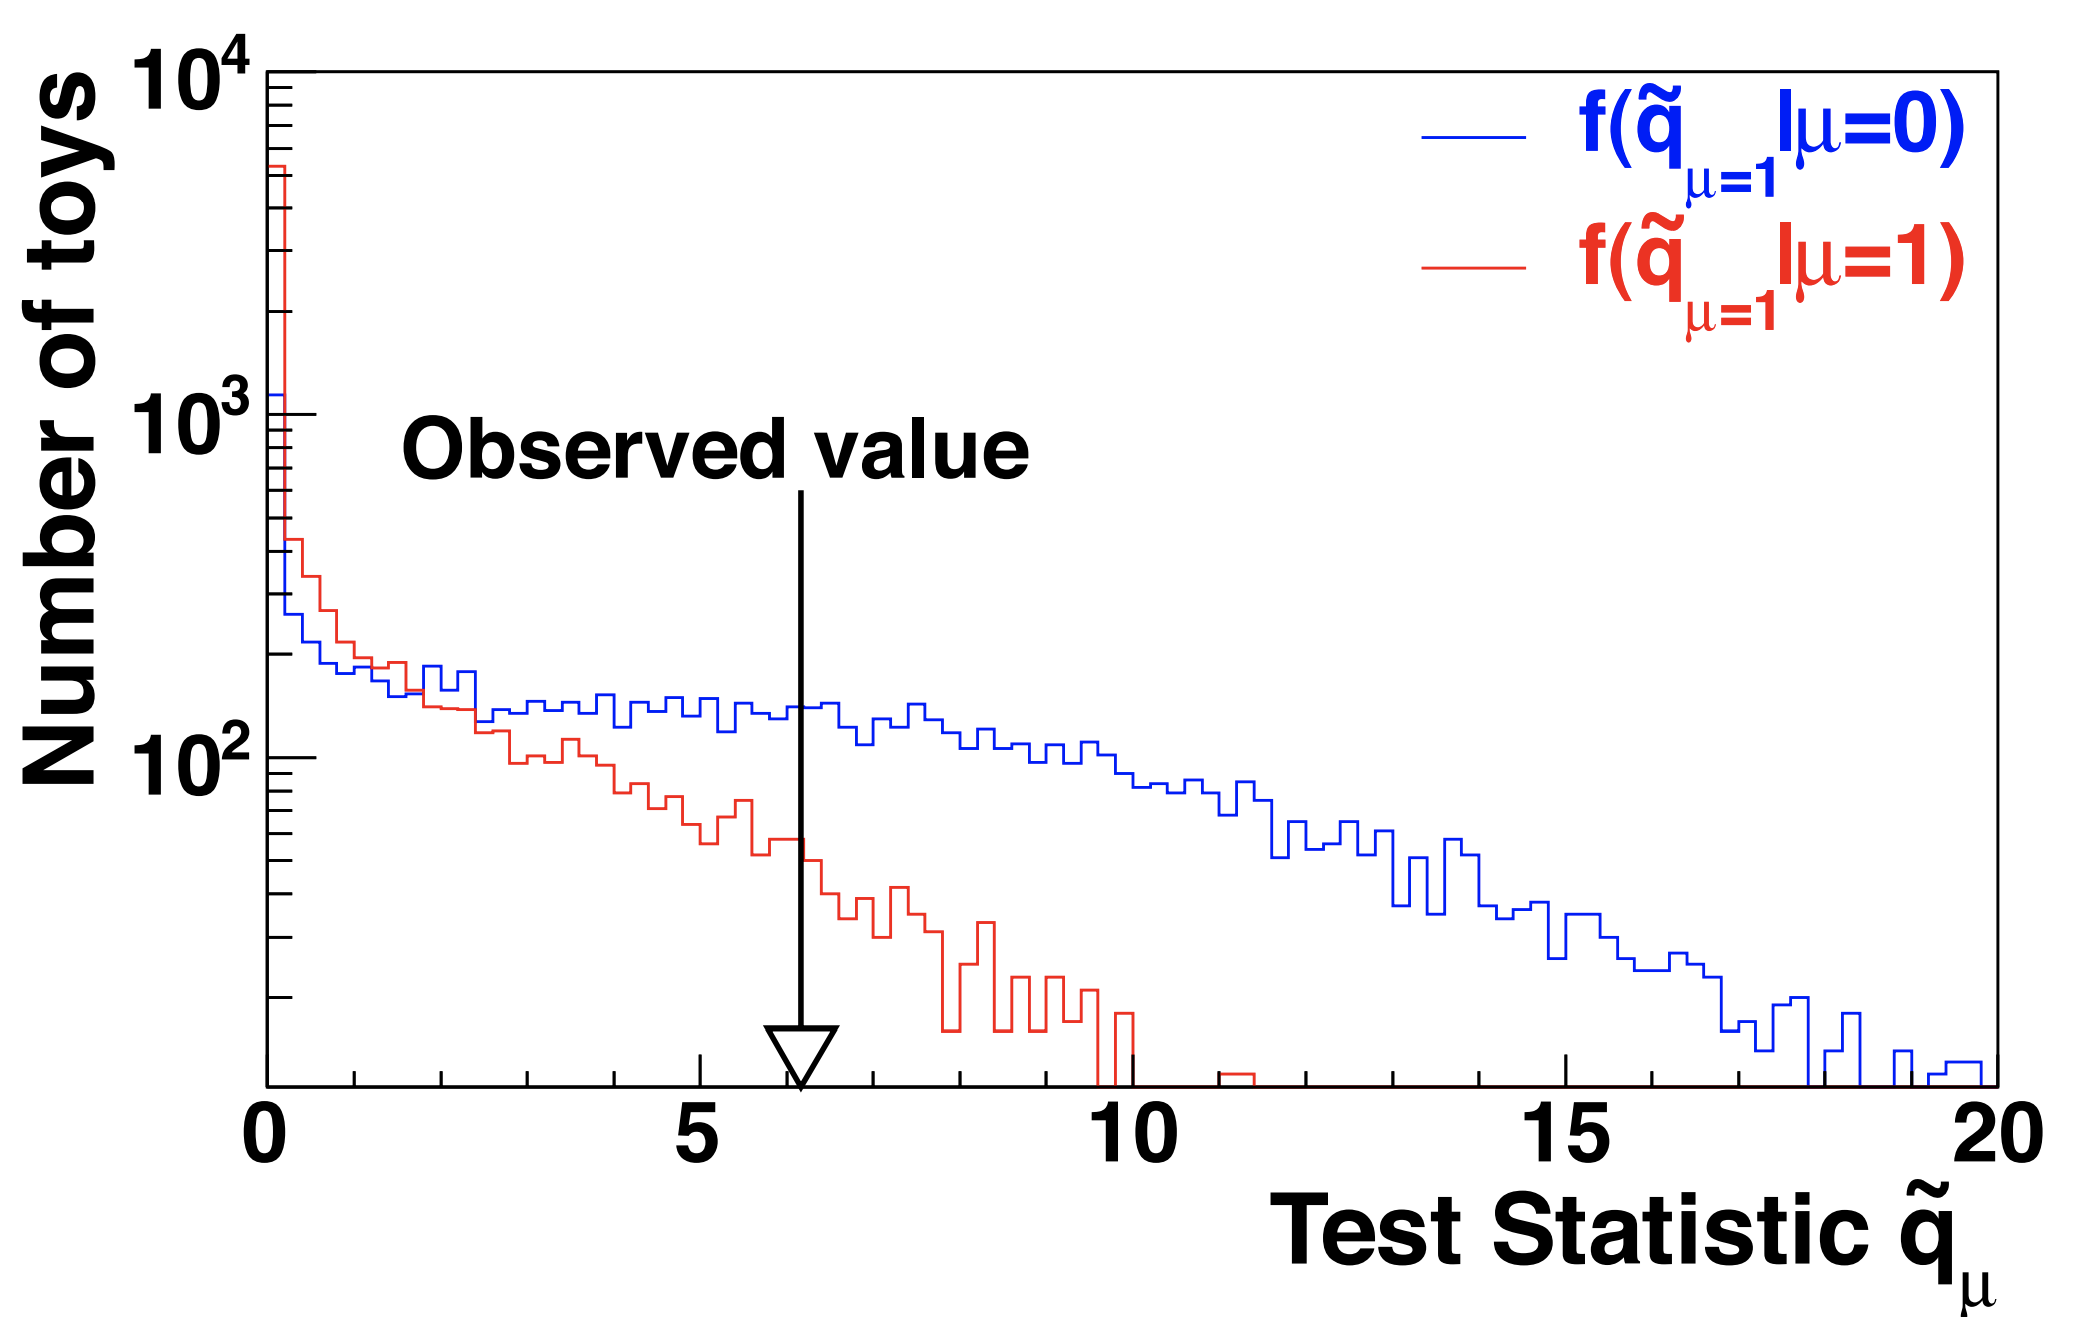
\includegraphics[width=0.7\textwidth,keepaspectratio]{figures_and_tables/cls/q_tilde.png}
  \caption{Example of $f(\tilde{q_{\mu}} \vert \mu, \hat{\theta}_{\mu}^{\text{obs}})$ $f(\tilde{q_{\mu}} \vert \mu=0, \hat{\theta}_{\mu = 0}^{\text{obs}})$ distributions generated with toy MC. Source:~\cite{cms_atlas_statistical_guidelines}.}
  \label{toy_mc_profile_likelihood_test}
\end{figure}

The $CL_s$ value is defined as:

\begin{equation}
  \label{cls_def}
  CL_s(\mu)=\frac{p_{s+b}(\mu)}{1-p_{b}},
\end{equation}
where:

\begin{equation}
  \label{cls_p_def1}
  p_{s+b}(\mu) = \int_{\tilde{q_{\mu}}^{\text{obs}}}^{\infty} f(\tilde{q_{\mu}} \vert \mu, \hat{\theta}_{\mu}^{\text{obs}}) \text{ }d\tilde{q_{\mu}}
\end{equation}
and
\begin{equation}
  \label{cls_p_def2}
  p_{b} = \int^{\tilde{q_{\mu}}^{\text{obs}}}_{-\infty} f(\tilde{q_{\mu}} \vert \mu=0, \hat{\theta}_{\mu = 0}^{\text{obs}}) \text{ }d\tilde{q_{\mu}}
\end{equation}

Scanning different values of $\mu$, within $0 \leqslant \hat{\mu} \leqslant \mu$, one would exclude the ones which $CL_s < \alpha$. CMS and ATLAS recommends a CL level ($1-\alpha$) of 95\%.

The main advantage of the $CL_s$ approach is that the presence of the denominator $1-p_{b}$ in~\ref{cls_def} penalizes the exclusion of regions in which the experiment is no sensitive. Figure~\ref{qtevDist} helps to illustrate this. One can notice that a small value of $p_{s+b}$ (yellow area) is balanced by large value of $p_{b}$ (green area). When the experimental sensitivity is higher, the two distributions tend to be far away from each other. Thus leading to a smaller compensation factor ($p_{b}$) and enhancing the chance of a exclusive $CL_s$ value.

\begin{figure}[htbp]
  \centering
  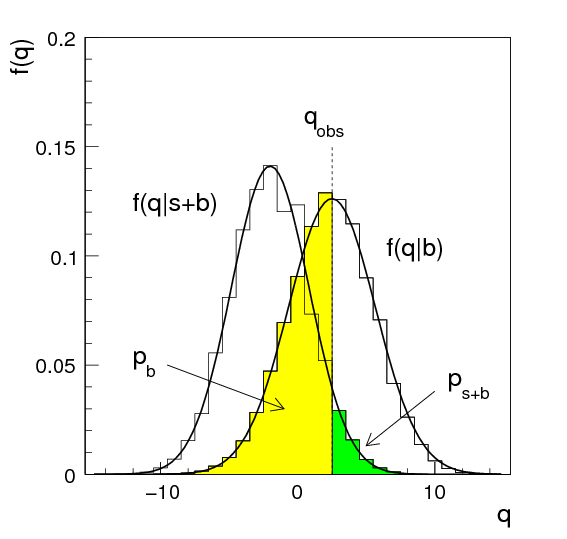
\includegraphics[width=0.5\textwidth,keepaspectratio]{figures_and_tables/cls/qtevDist.png}
  \caption{Example of $f(\tilde{q_{\mu}} \vert \mu, \hat{\theta}_{\mu}^{\text{obs}})$ $f(\tilde{q_{\mu}} \vert \mu=0, \hat{\theta}_{\mu = 0}^{\text{obs}})$ distributions generated with toy MC. In the figure, $q$ must be read as $\tilde{q}$. The green area shows the $p_{s+b}$ defined in~\ref{cls_p_def1}, while the yellow one shows $p_{b}$ defined in~\ref{cls_p_def2}. Source:~\cite{asymptotic_cls}.}
  \label{qtevDist}
\end{figure}

The expected upper limit and its $\pm 1 \sigma$ and $\pm 2 \sigma$ are determined by generating a large number of toy mc events, for the background-only model ($\mu = 0$), with nuisances free to float, and for each simulation finding $\mu_{95\%}$, which defines the confidence level. Once enough samples are generated, one should scan, from left to right, the cumulative distribution of $\mu_{95\%}$. The median defines the expected value and the quantiles for 16\%, 84\% and 2.5\%, 97.5\% defines the $\pm 1 \sigma$ and $\pm 2 \sigma$, respectively.

\subsection{Branching fraction upper limits}
\label{sec:results}
The results are summarized on table \ref{tab:UpperLimits_Cat123}.

\begin{table}[ht]
\begin{center}
\caption{Summary table for the limits on branching ratio of $\mathrm{Z}\to\Upsilon(1S,2S,3S)\gamma$ and $\mathrm{H}\to\Upsilon(1S,2S,3S)\gamma$ decays.}
%\resizebox{.5\width}{!}{\begin{tabular}{l|llll}
\multicolumn{4}{c}{95\% C.L. Upper Limit} \\
\hline
\hline
& \multicolumn{3}{c}{$\mathcal{B}(Z \rightarrow \Upsilon\gamma)$ $[\times10^{-6}]$}      \\
\cline{2-4}
&  $\Upsilon(1S)$ & $\Upsilon(2S)$ & $\Upsilon(3S)$  \\
\hline
Expected     & $6.4^{+3.1}_{-2.0}$ &  $8.3^{+4.0}_{-2.5}$  & $8.0^{+3.9}_{-2.4}$            \\
Observed     & 9.0 &  12.3  & 11.4      \\
\hline
SM Prediction $[\times10^{-8}]$ & 4.8  &  2.4  & 1.9      \\
\hline
\hline
& \multicolumn{3}{c}{$\mathcal{B}(H \rightarrow \Upsilon\gamma)$ $[\times10^{-4}]$}       \\
\cline{2-4}
&  $\Upsilon(1S)$ & $\Upsilon(2S)$ & $\Upsilon(3S)$ &   \\
\hline
Expected     & $12.5^{+6.1}_{-3.9}$ &  $14.6^{+7.1}_{-4.5}$  & $13.6^{+6.6}_{-4.2}$        \\
Observed     & 11.5 &  13.6  & 12.7     \\
\hline
SM Prediction $[\times10^{-9}]$ & 5.2  &  1.4  & 0.9      \\
\hline
\hline
\end{tabular}

}
% \begin{tabular}{l|llll}
\multicolumn{4}{c}{95\% C.L. Upper Limit} \\
\hline
\hline
& \multicolumn{3}{c}{$\mathcal{B}(Z \rightarrow \Upsilon\gamma)$ $[\times10^{-6}]$}      \\
\cline{2-4}
&  $\Upsilon(1S)$ & $\Upsilon(2S)$ & $\Upsilon(3S)$  \\
\hline
Expected     & $6.4^{+3.1}_{-2.0}$ &  $8.3^{+4.0}_{-2.5}$  & $8.0^{+3.9}_{-2.4}$            \\
Observed     & 9.0 &  12.3  & 11.4      \\
\hline
SM Prediction $[\times10^{-8}]$ & 4.8  &  2.4  & 1.9      \\
\hline
\hline
& \multicolumn{3}{c}{$\mathcal{B}(H \rightarrow \Upsilon\gamma)$ $[\times10^{-4}]$}       \\
\cline{2-4}
&  $\Upsilon(1S)$ & $\Upsilon(2S)$ & $\Upsilon(3S)$ &   \\
\hline
Expected     & $12.5^{+6.1}_{-3.9}$ &  $14.6^{+7.1}_{-4.5}$  & $13.6^{+6.6}_{-4.2}$        \\
Observed     & 11.5 &  13.6  & 12.7     \\
\hline
SM Prediction $[\times10^{-9}]$ & 5.2  &  1.4  & 0.9      \\
\hline
\hline
\end{tabular}



\begin{tabular}{l|llll}
\multicolumn{4}{c}{95\% C.L. Upper Limit} \\
\hline
\hline
& \multicolumn{3}{c}{$\mathcal{B}(Z \rightarrow \Upsilon\gamma)$ $[\times10^{-6}]$}      \\
\cline{2-4}
&  $\Upsilon(1S)$ & $\Upsilon(2S)$ & $\Upsilon(3S)$  \\
\hline
Expected     & $1.6^{+0.8}_{-0.5}$ &  $2.0^{+1.0}_{-0.6}$  & $1.8^{+1.0}_{-0.6}$            \\
Observed     & 2.9 &  2.7  & 1.4      \\
\hline
SM Prediction $[\times10^{-8}]$ & 4.8  &  2.4  & 1.9      \\
\hline
\hline
& \multicolumn{3}{c}{$\mathcal{B}(H \rightarrow \Upsilon\gamma)$ $[\times10^{-4}]$}       \\
\cline{2-4}
&  $\Upsilon(1S)$ & $\Upsilon(2S)$ & $\Upsilon(3S)$ &   \\
\hline
Expected     & $7.3^{+4.0}_{-2.4}$ &  $8.1^{+4.6}_{-2.8}$  & $6.8^{+3.9}_{-2.3}$        \\
Observed     & 6.9 &  7.4  & 5.8     \\
\hline
SM Prediction $[\times10^{-9}]$ & 5.2  &  1.4  & 0.9      \\
\hline
\hline
\end{tabular}
	
\label{tab:UpperLimits_Cat123}
\end{center}
\end{table}

The observed(expected) exclusion limit at $95\%$ confidence level on the $\mathcal{B}(\mathrm{Z}\to\Upsilon(1S,2S,3S)\gamma)=$ 2.9, 2.7, 1.4 ($1.6^{+0.8}_{-0.5}$,  $2.0^{+1.0}_{-0.6}$, $1.8^{+1.0}_{-0.6}$)$\times 10^{-6}$, and on the $\mathcal{B}(\mathrm{H}\to\Upsilon(1S,2S,3S)\gamma)=$ 6.9, 7.4, 5.8 ($7.3^{+4.0}_{-2.4}$,  $8.1^{+4.6}_{-2.8}$, $6.8^{+3.9}_{-2.3}$)$\times 10^{-4}$.

As stated before, this analysis was done, for the Z decay, taking into account a mutually excludent categorization of events, based on the reconstructed photon properties ($\eta_{SC}$ and R9 value), as described in section~\ref{sec:categorization}. 

At table~\ref{tab:UpperLimits_Cat0} we present the results obtained when there is no categorization of events (Inclusive category).

\begin{table}[ht]
\begin{center}
\caption{Summary table for the limits on branching ratio of $\mathrm{Z}\to\Upsilon(1S,2S,3S)\gamma$, for the two possible categorization scenarios.}
%\resizebox{.5\width}{!}{\begin{tabular}{l|llll}
\multicolumn{4}{c}{95\% C.L. Upper Limit} \\
\hline
\hline
& \multicolumn{3}{c}{$\mathcal{B}(Z \rightarrow \Upsilon\gamma)$ $[\times10^{-6}]$}      \\
\cline{2-4}
&  $\Upsilon(1S)$ & $\Upsilon(2S)$ & $\Upsilon(3S)$  \\
\hline
Expected     & $6.4^{+3.1}_{-2.0}$ &  $8.3^{+4.0}_{-2.5}$  & $8.0^{+3.9}_{-2.4}$            \\
Observed     & 9.0 &  12.3  & 11.4      \\
\hline
SM Prediction $[\times10^{-8}]$ & 4.8  &  2.4  & 1.9      \\
\hline
\hline
& \multicolumn{3}{c}{$\mathcal{B}(H \rightarrow \Upsilon\gamma)$ $[\times10^{-4}]$}       \\
\cline{2-4}
&  $\Upsilon(1S)$ & $\Upsilon(2S)$ & $\Upsilon(3S)$ &   \\
\hline
Expected     & $12.5^{+6.1}_{-3.9}$ &  $14.6^{+7.1}_{-4.5}$  & $13.6^{+6.6}_{-4.2}$        \\
Observed     & 11.5 &  13.6  & 12.7     \\
\hline
SM Prediction $[\times10^{-9}]$ & 5.2  &  1.4  & 0.9      \\
\hline
\hline
\end{tabular}

}
% \begin{tabular}{l|llll}
\multicolumn{4}{c}{95\% C.L. Upper Limit} \\
\hline
\hline
& \multicolumn{3}{c}{$\mathcal{B}(Z \rightarrow \Upsilon\gamma)$ $[\times10^{-6}]$}      \\
\cline{2-4}
&  $\Upsilon(1S)$ & $\Upsilon(2S)$ & $\Upsilon(3S)$  \\
\hline
Expected     & $6.4^{+3.1}_{-2.0}$ &  $8.3^{+4.0}_{-2.5}$  & $8.0^{+3.9}_{-2.4}$            \\
Observed     & 9.0 &  12.3  & 11.4      \\
\hline
SM Prediction $[\times10^{-8}]$ & 4.8  &  2.4  & 1.9      \\
\hline
\hline
& \multicolumn{3}{c}{$\mathcal{B}(H \rightarrow \Upsilon\gamma)$ $[\times10^{-4}]$}       \\
\cline{2-4}
&  $\Upsilon(1S)$ & $\Upsilon(2S)$ & $\Upsilon(3S)$ &   \\
\hline
Expected     & $12.5^{+6.1}_{-3.9}$ &  $14.6^{+7.1}_{-4.5}$  & $13.6^{+6.6}_{-4.2}$        \\
Observed     & 11.5 &  13.6  & 12.7     \\
\hline
SM Prediction $[\times10^{-9}]$ & 5.2  &  1.4  & 0.9      \\
\hline
\hline
\end{tabular}



\begin{tabular}{l|llll}
\multicolumn{4}{c}{95\% C.L. Upper Limit - $\mathcal{B}(Z \rightarrow \Upsilon\gamma)$ $[\times10^{-6}]$} \\
\hline
\hline
& \multicolumn{3}{c}{without categorization}      \\
\cline{2-4}
&  $\Upsilon(1S)$ & $\Upsilon(2S)$ & $\Upsilon(3S)$  \\
\hline
Expected     & $1.7^{+0.9}_{-0.5}$ &  $2.1^{+1.1}_{-0.7}$  & $1.9^{+1.0}_{-0.6}$            \\
Observed     & 2.6 &  2.3  & 1.2      \\
\hline
\hline
& \multicolumn{3}{c}{with categorization}      \\
\cline{2-4}
&  $\Upsilon(1S)$ & $\Upsilon(2S)$ & $\Upsilon(3S)$  \\
\hline
Expected     & $1.6^{+0.8}_{-0.5}$ &  $2.0^{+1.0}_{-0.6}$  & $1.8^{+1.0}_{-0.6}$            \\
Observed     & 2.9 &  2.7  & 1.4      \\
\hline
\hline
\end{tabular}
	
\label{tab:UpperLimits_Cat0}
\end{center}
\end{table}

It is worth to remember that the categorization takes places only for the Z decay. For the Higgs decay, no categorization is imposed.

By taking, or not, into account any categorization, the numbers presented in both tables (\ref{tab:UpperLimits_Cat123} and \ref{tab:UpperLimits_Cat0}), are compatible within themselves and with the results published by the ATLAS collaboration~\cite{atlas_paper_2018:2018txb}. Our interpretation to the lack of improvement of the no categorization scenario with respect to the categorized one, is that, the collected statistics, after full selection, is so small, that the categorization just jeopardize the amount of events available. 

